\chapter{Physics-Informed Neural Networks (PINNs)}
\section{Overview}
\label{sec:pinns_overview}

Physics-informed neural networks can be considered as an alternative approach to conventional partial
differential equation (PDE) solvers. 
The general idea is to solve problems by minimizing the loss function constructed from PDEs where data
is limited. Compared to conventional solvers, PINNs

\begin{itemize}
    \item are mesh-free.
    \item can efficiently handle unstructured or irregular domains \cite{lu2021physics}.
    \item can be applied to solve also \textit{inverse} problems.
\end{itemize}

%-------------------------------------------------------------------------------------------------------------------
\section{Formulation of a PINN}
\label{sec:pinns_formulation}

\noindent Consider a partial differential equation as 

\begin{equation}
    \label{eq:governing}
    \frac{\partial u}{\partial t}+\mathcal{N}[u ; \lambda]=0, x \in \Omega, t \in [0,\mathcal{T}]
\end{equation}

\noindent where $u(t,x)$ is the latent solution with time $t \in [0,\mathcal{T}]$ and a spatial variable
$x \in \Omega$, $\mathcal{N}[u;\lambda]$ is the nonlinear differential operator
with the coefficient $\lambda$, and $\Omega$ is a subset of $\mathbb{R}^{D}$.

The conventional methods to solve Eq. \ref{eq:governing} are either analytical or numerical. The analytical solutions are 
not always feasible and numerical methods are expensive. The PINNs approach can be considered more feasible than analytical
methods and less expensive than numerical methods. 
The physics-informed neural network estimates the solution $u(t,x)$ and the physics-enhanced part evaluates
the given partial differential equation using the estimated solution. As shown in Fig. \ref{fig:pinn_arch}, the physics-informed
neural network predicts the solution $u(x,t)$ by using fully connected layers with nonlinear activation functions,
denoted as $\sigma$. The physics-enhanced part evaluates the chosen PDE, denoted as $f(x)$, using the higher derivatives
of the solution $u(x,t)$, denoted here $d_{x}, d_{xx}$ and $d_{t}$, with respect to space ($x$) and time ($t$), and the identity 
matrix of $u$. Since the solution is known on the boundaries and the approximated solution must fulfill the governing PDE, the loss
can be computed using a cost function, i.e. mean squared error. If the solution is not converged, the weights of the neural network
are updated using back-propagation to estimate the new solution, until the given convergence limit is reached. 


\begin{figure}[thbp]
    \centering
    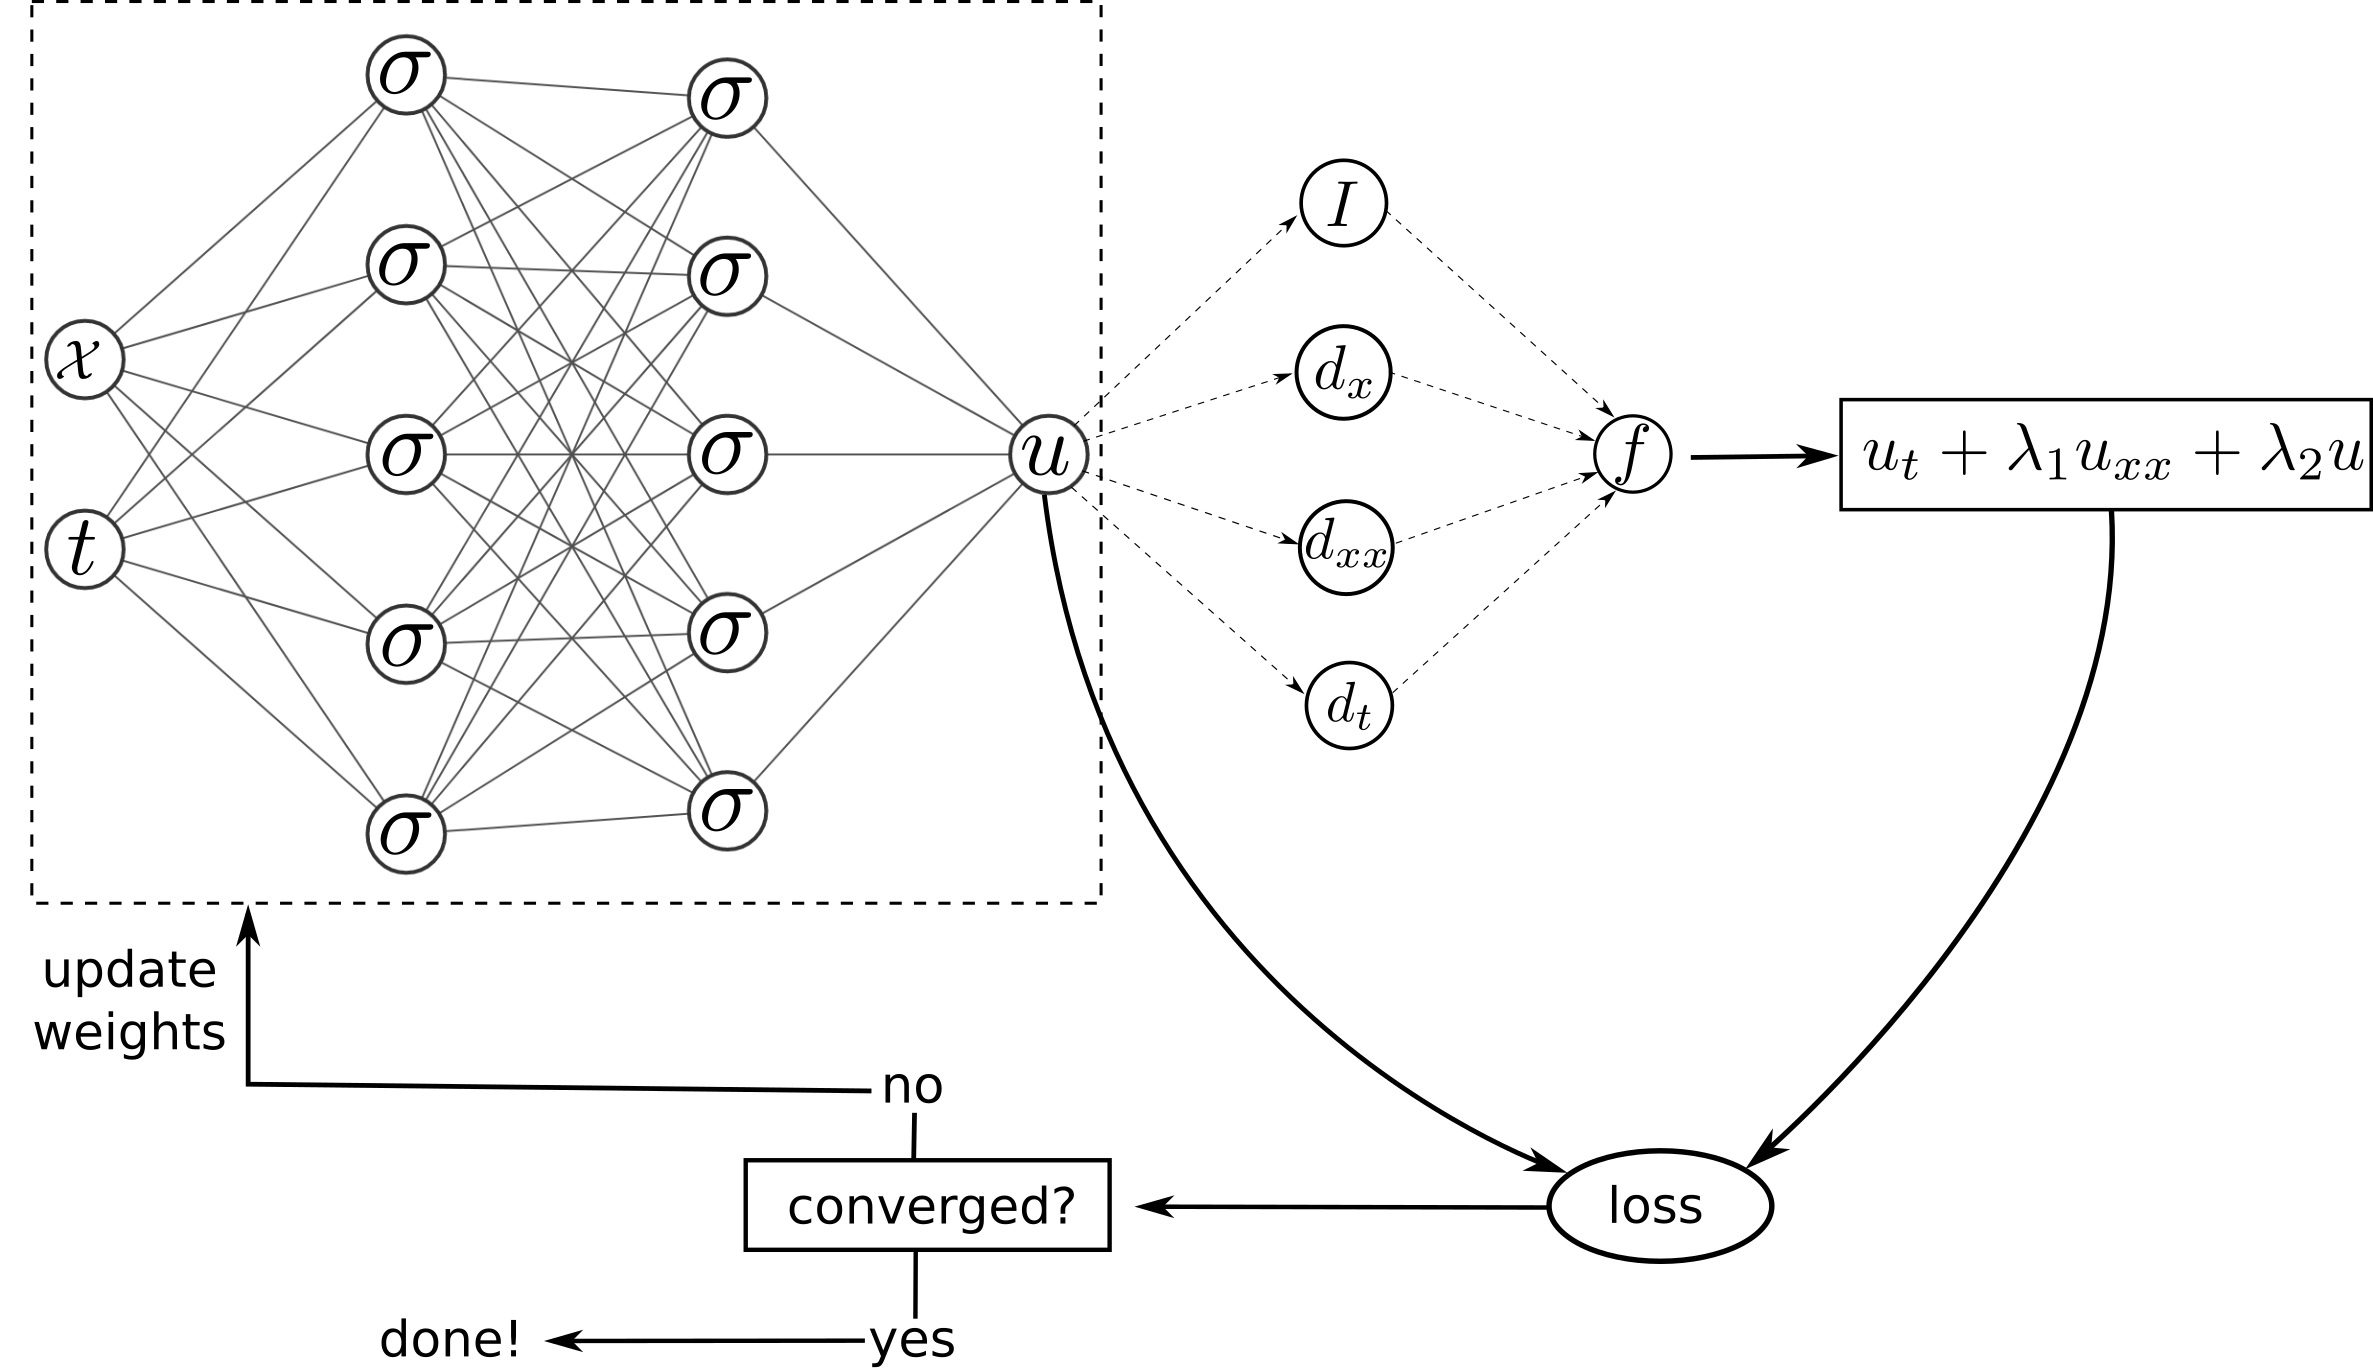
\includegraphics[scale=0.59]{pinn.png}  
    \caption{The visionary representation of physics-informed neural network for an arbitrary space-time dependent partial
    differential equation. }
    \label{fig:pinn_arch}
\end{figure}

Compared to classical neural networks, the loss function of a PINN has three terms:

\begin{equation}
    \label{eq:total_loss_compact}
    L = E_{u} +  E_{0} + E_{f}
\end{equation}

\noindent The first term, denoted as $E_{u}$, calculates the error for the approximated solution on the known
boundaries. In the case of a one dimensional non-linear heat equation subjected to the following 
homogenous Neumann boundary condition

\begin{equation}
    \label{eq:neumann}
    \frac{\partial u(x=1, t)}{\partial x}=h,
\end{equation}

\noindent the Dirichlet boundary condition

\begin{equation}
    \label{eq:dirichlet}
     u(x=0,t)=g,
\end{equation}

\noindent $E_{u}$ term is calculated as

\begin{equation}
    \label{eq:total_loss}
    E_{u} = E_{Neumann} + E_{Dirichlet},
\end{equation}

\noindent where

\begin{equation}
    \label{eq:Neumann_pinn}   
    E_{\text {Neumann}}=\frac{1}{N_{b}} \sum_{i=1}^{N_{b}}\left(\frac{\partial}{\partial x} u_{P}\left(x_{b}^{i}, t_{b}^{i} \right)-h\right)^{2}
\end{equation}

\noindent  enforces the homogenous Neumann boundary condition (refer to \ref{eq:neumann}) by penalizing the error between
the derivative of the predicted solution, denoted as $\frac{\partial}{\partial x} u_{P}\left(x_{b}^{i}, t_{b}^{i}\right)$, 
and the given Neumann
boundary condition $h$ at $N_{b}$ random
points $\left\{x_{b}^{i}, t_{b}\right\}_{i=1}^{N_{b}}$ on the boundary $x_{b} = 1$.

\noindent The term, $E_{Dirichlet}$ of the Eq. \ref{eq:total_loss}

\begin{equation}
    \label{eq:Dirichlet_pinn}      
    E_{\text {Dirichlet}}=\frac{1}{N_{b}} \sum_{i=1}^{N_{b}}\left(u_{P}\left(x_{b}^{i}, t_{b}^{i} \right)-g\right)^{2}
\end{equation}

\noindent enforces the Dirichlet boundary condition according Eq. \ref{eq:dirichlet}  by penalizing the error 
between approximated solution $u_{P}(x_{b}^{i}, t_{b}^{i})$ and prescribed Dirichlet boundary condition $g$ 
at $N_{b}$ random points $\left\{x_{b}^{i}, t_{b} \right\}_{i=1}^{N_{b}}$ on the boundary $x_{b} = 0$. 

\vspace{4mm}

\noindent The initial condition loss, $E_{0}$ of the Eq. \ref{eq:total_loss_compact}

\begin{equation}
    \label{eq:Initial_pinn}  
    E_{0}=\frac{1}{N_{0}} \sum_{i=1}^{N_{0}}\left(u_{P}\left(x_{0}^{i}, 0 \right)-u_{0}^{i}\right)^{2},
\end{equation}

\noindent with the following initial condition
\begin{equation}
    \label{eq:initial}
    u(x, t=0)=u_{0},
\end{equation}

\noindent enforces the initial conditions at $N_{0}$ random points 
$\left\{x_{0}^{i}, t_{b} \right\}_{i=1}^{N_{0}}$ at initial time $t_{b}=0$

\vspace{4mm}

The loss functions $E_{u}$ and $E_{0}$ contain only the loss on the known boundaries and
on the known initial conditions, respectively.

On the other hand, the final term of the Eq. \ref{eq:total_loss_compact}

\begin{equation}
    \label{eq:res_loss}   
    E_{\text {f}}=\frac{1}{N_{f}} \sum_{i=1}^{N_{f}}\left(\frac{\partial}{\partial t} u_{P}\left(x_{f}^{i}, t_{b}^{i} \right)-\mathcal{N}[u_{P}(x_{b}^{i}, t_{b}^{i})]\right)^{2}
\end{equation}

\noindent imposes the given partial differential equation at every random collocation point inside the domain by penalizing the estimated 
left-hand side and the known right-hand side of the governing equation. Since PINNs are mesh-free, the distribution of 
collocation points can be uniform or random.

After calculation of the loss terms, weights of the architecture is updated using back-propagation with the help of a optimization function,
i.e. stochastic gradient descent, Adam etc. 

\section{General remarks regarding PINNs}
\begin{itemize}
    \item A PINN is mesh-free so it can handle unstructured or irregular domains.
    \item PINNs can be deployed on both forward and inverse problems. In forward problems, they can find the hidden solution
    $u(x,t)$ 
    where the coefficients $\lambda$ are known (Eq. \ref{eq:governing}) or discover
    the parameters $\lambda$ using the provided solution, which are known as inverse problems. This approach
    is called also as data-driven identification.
    \item Depending on the type of the governing equation, they can be used on a wide variety of problems ranging from biological
    systems (reconstruction clinical magnetic resonance imaging (MRI) data) to the governing equations of continuum mechanics.
    \item Since the governing equations of the problem are involved in the learning process, PINNs can learn even data is limited.
    \item The derivatives of the network prediction $u_{P}$ with respect to space ($x$) and time ($t$) can be easily and
    efficiently computed by the automatic differentiation capabilities implemented in many deep learning tool kits, i.e. Tensorflow 
    \cite{abadi2016tensorflow} and 
    Pytorch \cite{NEURIPS20199015}.
    
\end{itemize}


















